% !TEX program = pdflatex
\documentclass[11pt,a4paper]{article}

% --------- Packages ---------------------------------------------------------
\usepackage[utf8]{inputenc}
\usepackage[T1]{fontenc}
\usepackage[english]{babel}
\usepackage{lmodern}
\usepackage[a4paper,margin=2.3cm]{geometry}
\usepackage{graphicx}
\usepackage{booktabs}
\usepackage{array}
\usepackage{amsmath,amssymb}
\usepackage{eurosym}
\usepackage{caption}
\usepackage{subcaption}
\usepackage{natbib}
\usepackage{hyperref}
\usepackage{microtype}
\usepackage{enumitem}
\usepackage{tabularx}
\usepackage{multirow}
\usepackage{float}
\usepackage{xcolor}

\hypersetup{
    colorlinks=true,
    linkcolor=blue!50!black,
    citecolor=blue!50!black,
    urlcolor=blue!60!black,
}

\bibliographystyle{abbrvnat}
\setcitestyle{authoryear,round}

\captionsetup{font=small,labelfont=bf}

% --------- Compact float spacing --------------------------------------------
\setlength{\textfloatsep}{8pt plus 2pt minus 2pt}
\setlength{\floatsep}{8pt plus 2pt minus 2pt}
\setlength{\intextsep}{8pt plus 2pt minus 2pt}
\setlength{\abovecaptionskip}{4pt}

% --------- Metadata ---------------------------------------------------------
\title{\textbf{Subsidising the Metro per passenger or per kilometre?\\
A calibrated translog cost function for the Barcelona Metro\\
(FMB-TMB), 2023--2025}}
\author{Carlo Vilches Cevallos \\
\small{Universitat de Barcelona} \\
\small{\texttt{cvilchce15@alumnes.ub.edu}}}
\date{\today}

% =============================================================================
\begin{document}
\maketitle

% --------- ABSTRACT ---------------------------------------------------------
\begin{abstract}
\noindent This paper calibrates the cost structure of the Barcelona Metro
(Ferrocarril Metropolit\`{a} de Barcelona, FMB) for 2023--2025 using a
multiproduct translog cost function on a line-year panel of 21 observations
(7 operating blocks $\times$ 3 fiscal years). Two items in the FMB
accounts---the Ifercat L9 concession fee and train leasing---jointly
represent about 29 per cent of total declared cost and have the character
of quasi-fixed contractual transfers rather than technological inputs. We
therefore model total cost as the additive decomposition
$C_{\text{total}}(Y,W,\text{inst.}) = C_{\text{tec}}(Y,W) + F_{\text{inst}}$,
where $C_{\text{tec}}$ is the translog cost function and $F_{\text{inst}}$
is the institutional component. Forcing $F_{\text{inst}}$ inside the
translog breaks Shephard concavity in 48 per cent of observations, a
direct empirical confirmation of the conceptual argument. Under the
calibrated technological model, returns to density are substantial
(RTD~$\approx 2.18$), under the calibrated parameters the marginal cost is
about 0.42~\euro{}/pax against an average cost of 0.91~\euro{}/pax
(MC/AC~$\approx 0.46$), and the Boiteux optimal subsidy is approximately
54 per cent of technological average cost. $F_{\text{inst}}$ contributes
roughly 0.38~\euro{}/pax system-wide and reflects institutional burden
rather than operational inefficiency: it represents around 70 per cent of
total cost in L9/L10 but only 8 per cent in L1--L5. Accounting separation
aligned with the spirit of Directive 2012/34/EU is not applied in FMB
consolidated accounts, biasing any efficiency or social cost--benefit
assessment.

\bigskip
\noindent\textbf{Keywords:} Translog cost function; urban rail; returns
to density; infrastructure access charge; optimal subsidy; Barcelona.\\
\textbf{JEL classification:} L92, L43, R41, H42.
\end{abstract}

% =============================================================================
\section{Introduction}
\label{sec:intro}

The economics of urban metro systems combines three features that the
literature regards as central for regulatory design: network structure,
sunk capital investment, and substantial returns to density. These features
justify operating subsidies, tariff regulation, and dedicated concession
contracts \citep{joskow2008,gagnepainivaldi2002}. Ferrocarril
Metropolit\`{a} de Barcelona, S.A.\ (FMB), the operating subsidiary of the
Barcelona Metro within the Transports Metropolitans de Barcelona (TMB)
group, exhibits an additional institutional feature of regulatory
relevance: lines L9 and L10---among the longest driverless automated metro
lines in Europe---are operated under an availability-based concession fee
paid to the public entity Infraestructures Ferrovi\`{a}ries de Catalunya
(Ifercat), a body of the Generalitat de Catalunya that owns the underlying
infrastructure. In 2023--2024 this fee exceeded 135~M\euro{} per year,
equivalent to 22--23 per cent of total recurrent cost, and it is designed
to recover approximately 8~billion~\euro{} of historical civil-works
investment over the asset life. L9/L10 carries roughly 6 per cent of
system passengers but generates the single largest institutional cost item
in the group accounts. A second contractual item---train leasing
(45--47~M\euro{} per year, around 6--7 per cent of total cost)---reflects
operationalised capital cost via long-term financial-lease agreements,
mainly for the renewal of the 6000/7000 fleet on lines L1, L3 and L5.

Despite the regulatory centrality of Barcelona within Spain, the empirical
literature has not quantified the elasticities of its cost function with a
methodology that can inform tariff or concession reform:
\citet{matasraymond2009} examines Spanish urban transport at the national
level without isolating the rail concession fee, and \citet{daraio2016}
reviews international metro frontiers without a Barcelona case. The
contribution of this paper is not to replicate the existence of density
economies, but to isolate the technological component of the cost function
from the institutional component and to demonstrate microeconomically that
the two must be analysed separately. We calibrate a translog cost function
$C_{\text{tec}}(Y,W)$ over the line-year panel under expenditure
minimisation, treat the contractual items (concession fee, leasing) as an
additive non-functional component $F_{\text{inst}}$, and show that forcing
$F_{\text{inst}}$ inside the translog produces concavity failure in 48 per
cent of observations and a 3.8$\times$ degradation in fit---direct
evidence that this is not a technological cost.

European rail-sector regulation has, since the early 1990s, progressively
required vertical separation between infrastructure managers and operators,
culminating in Directive 2012/34/EU \citep{directive2012}, which
establishes the single European railway area and mandates accounting
separation between the two functions. Urban metro systems are not formally
within the scope of this directive, but its underlying economic logic---that
mixing infrastructure-related charges with operating costs distorts
efficiency signals and biases regulatory comparisons---applies a fortiori
to systems such as TMB where the infrastructure-access charge represents
nearly a quarter of total declared cost. This paper provides the
microeconomic foundation for that logic and quantifies what it implies for
the Barcelona Metro.

The paper is organised as follows. Section~\ref{sec:marco} sets out the
theoretical framework and the connection with network regulation.
Section~\ref{sec:datos} describes the data and the construction of the
panel. Section~\ref{sec:calib} presents the calibration strategy,
including the treatment of non-technological components
(Section~\ref{sec:treatment}) and the production technology and
substitution margins (Section~\ref{sec:margins}). Section~\ref{sec:resultados}
reports the results under the four hypotheses, with the decomposition
evidence in Section~\ref{sec:h3}. Section~\ref{sec:robustez} consolidates
the robustness analyses. Section~\ref{sec:politica} discusses regulatory
and policy implications. Section~\ref{sec:limit} acknowledges limitations;
Section~\ref{sec:concl} concludes.

\medskip
\begin{figure}[H]
    \centering
    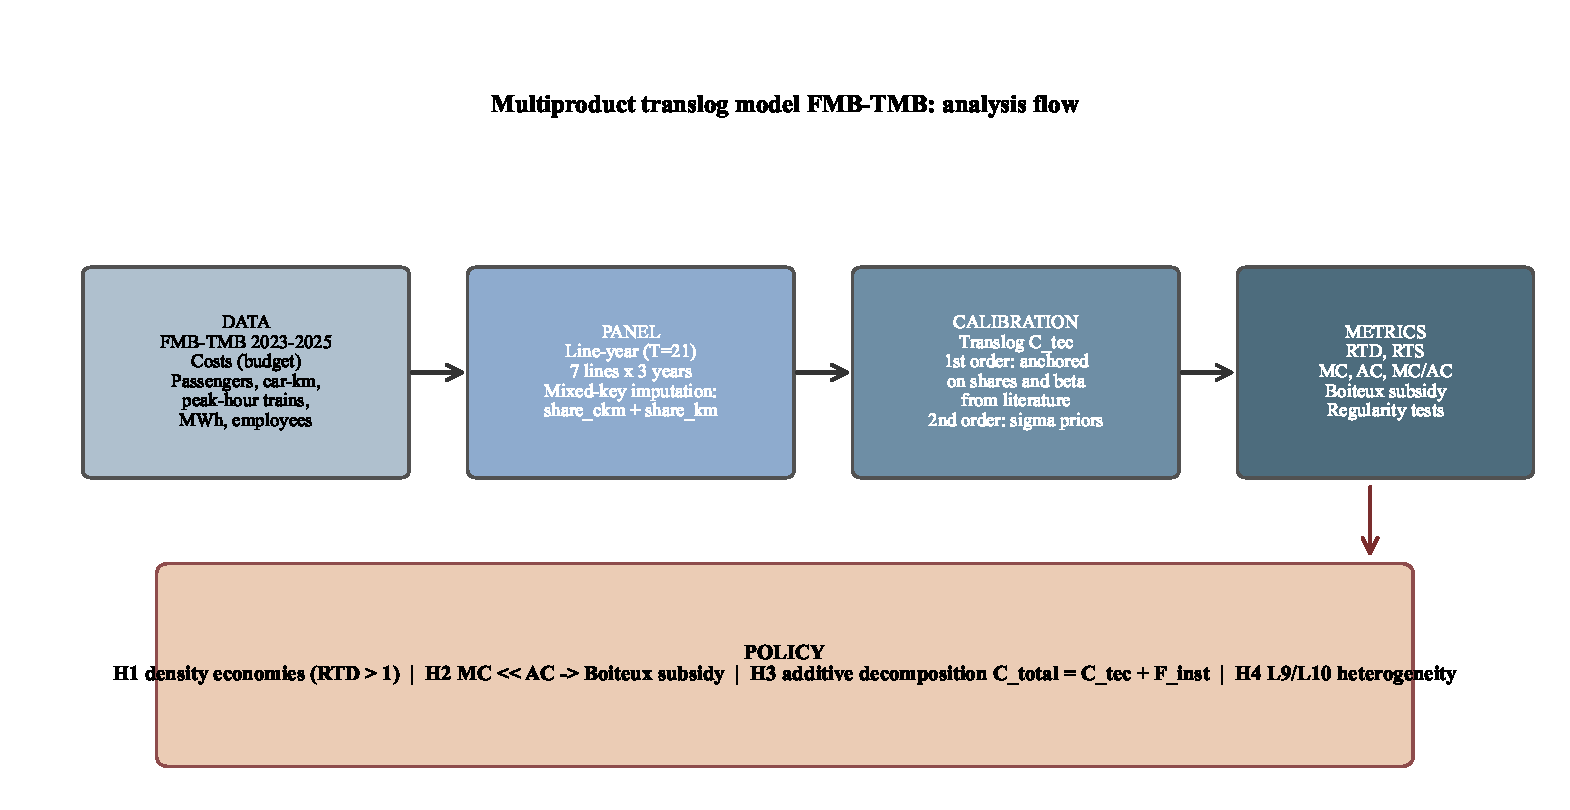
\includegraphics[width=0.72\linewidth]{../outputs/figures/fig8_conceptual.pdf}
    \caption{Methodological flow: data $\rightarrow$ line-year panel
    $\rightarrow$ calibration $\rightarrow$ metrics $\rightarrow$ policy.}
    \label{fig:conceptual}
\end{figure}

% =============================================================================
\section{Theoretical framework}
\label{sec:marco}

\subsection{Multiproduct translog cost function}
The translog cost function \citep{cjl1973} is a second-order approximation
to an arbitrary cost function. With two outputs---passengers $Y_1$ and
service car-km $Y_2$---and three inputs---labour $L$, energy $E$ and an
aggregate of other inputs $O$---the specification is
\begin{align}
\ln C &= \alpha_0 + \sum_{i\in\{L,E,O\}} \alpha_i \ln W_i
         + \sum_{k=1,2} \beta_k \ln Y_k
         + \tfrac{1}{2}\sum_{i,j} \gamma_{ij}\ln W_i \ln W_j \notag\\
      &\qquad + \tfrac{1}{2}\sum_{k,l} \delta_{kl}\ln Y_k \ln Y_l
         + \sum_{i,k} \rho_{ik}\ln W_i \ln Y_k + \lambda t + \varepsilon.
\label{eq:translog}
\end{align}
\emph{Linear homogeneity in prices} imposes $\sum_i \alpha_i = 1$,
$\sum_j \gamma_{ij}=0$ and $\sum_i \rho_{ik}=0$. The \emph{symmetry}
restrictions $\gamma_{ij}=\gamma_{ji}$ and $\delta_{kl}=\delta_{lk}$ are
assumed. Normalising by the price of the \emph{other-inputs} aggregate
$W_O$ (the numeraire) and centring all variables on the sample geometric
mean, the cost equation is rewritten in terms of the relative prices
$W_L/W_O$ and $W_E/W_O$ only.

\subsection{Returns to density, scale and scope}
Following \citet{caves1984}, returns to density are defined as the
reciprocal of the cost--passenger elasticity (network held fixed):
\begin{equation}
\text{RTD} \;=\; \frac{1}{\partial \ln C / \partial \ln Y_1}
       \;=\; \frac{1}{\varepsilon_{Y_1}} ,
\label{eq:rtd}
\end{equation}
and returns to scale as $\text{RTS}=1/(\varepsilon_{Y_1}+\varepsilon_{Y_2})$.
For a translog function the elasticities \emph{vary by observation}
because of the interaction terms $\delta_{kl}$ and $\rho_{ik}$. A value
RTD~$>1$ indicates increasing returns to network \emph{utilisation}:
adding passengers to a given car-km supply reduces average cost.

\subsection{Cost shares and Shephard's lemma}
By the lemma of \citet{shephard1953} and the cost--production duality of
\citet{diewert1971}, input cost shares satisfy
$s_i = \partial \ln C / \partial \ln W_i$ and, in a translog,
\begin{equation}
s_i \;=\; \alpha_i + \sum_j \gamma_{ij}\ln W_j + \sum_k \rho_{ik} \ln Y_k .
\end{equation}
The Allen--Uzawa elasticities of substitution \citep{uzawa1962} are then
$\sigma_{ij} = 1 + \gamma_{ij}/(s_i s_j)$ for $i\neq j$.

\subsection{Connection with network regulation}
When marginal cost is well below average cost---a typical feature of
network industries---marginal-cost pricing generates structural deficits.
The rule of \citet{boiteux1956} establishes that the optimal tariff depends
on the elasticity of demand, but the \emph{level} of the public subsidy
required to close the gap is $1 - \text{MC}/\text{AC}$. This logic is part
of the body of public-finance theory of urban
transport~\citep{small2007,pigou1920,allais1947} and is the foundation of
the metropolitan operating subsidy in Barcelona.

% =============================================================================
\section{Data and panel construction}
\label{sec:datos}

\subsection{Sources}
Financial figures come from the quarterly tracking of the FMB budget
published by the TMB transparency portal for 2023 (Q4), 2024 (Q4) and
2025 (Q3, partial), cross-checked with the audited FMB 2023 accounts and
Note 18 of the audited 2024 TMB Group report (which isolates the FMB
subsidiary). Operating indicators---passengers per line, car-km, place-km,
employees, peak-hour trains and network length---come from the TMB
\emph{Basic data} fact sheets. Physical electricity consumption is taken
from the 2024 TMB Sustainability Report (255{,}413~MWh in 2023; 239{,}402~MWh
in 2024).\footnote{Operating labour in the audited accounts
(240.482~M\euro{} in 2023) differs by 0.5 per cent from operating labour
in the budget (239.328~M\euro{}). We use the budget series for temporal
consistency with 2024 and 2025.}

\subsection{Line-year panel}
The granularity of the published financial statements is the consolidated
subsidiary (FMB), not the individual line. With three years of aggregate
data the variability matrix of the translog function is structurally
ill-conditioned (see Section~\ref{sec:robustez}). We therefore construct
a \emph{line-year panel} of 21 observations by mixed-key imputation of
the FMB cost categories to 7 operating blocks: L1, L2, L3, L4, L5,
L9/L10~North and L9/L10~South. L11 and the Funicular are excluded on
grounds of technological heterogeneity.

\subsection{Theoretical justification of the imputation key}
The choice of imputation key is the central methodological decision.
\citet{small2007} and \citet{nashpreston1995} argue that operating costs
of urban rail---driving, supervision, light maintenance, traction
energy---scale with \emph{service supply} (car-km), not with realised
demand (passengers). Imputing every cost item proportionally to
passengers would mechanically yield a cost--passenger elasticity equal to
unity and $\text{RTD}=1$. We therefore adopt:

\begin{itemize}[leftmargin=*,topsep=2pt]
\item Operating labour, energy, supplies, external services and train
leasing are imputed by the car-km share,
$\text{share\_ckm}_{l,t}=\text{peak\_trains}_{l,t}\times
\text{km\_line}_l$, normalised at the system level.
\item Net depreciation is imputed by the share of network length
(\emph{share\_km}), reflecting installed physical capital.
\item The Ifercat L9 concession fee is allocated entirely to L9/L10,
split between the North and South blocks in proportion to their passenger
share.
\end{itemize}

\subsection{Treatment of 2025 (partial)}
Published FMB accounts for 2025 cover January--September. We annualise all
items by multiplying by $12/9$. For energy, the Q3 \euro{}/kWh price is
not a reliable representation of the annual closing figure; we impute the
2024 MWh and price (0.0815~\euro{}/kWh; 239{,}402~MWh). The workforce is
not annualised (it is an end-of-period stock).

\subsection{Variable definitions}
\begin{table}[H]
\centering
\caption{Operating definitions.}
\label{tab:defs}
\small
\begin{tabularx}{\linewidth}{l X}
\toprule
Variable & Definition \\
\midrule
$C_{\text{tec}}$ & Technological cost: labour + energy + supplies +
external services + net depreciation. \\
$F_{\text{inst}}$ & Institutional component: train leasing + Ifercat L9
concession fee. \\
$C_{\text{total}}$ & Total declared cost: $C_{\text{tec}} + F_{\text{inst}}$. \\
$Y_1$            & Passengers (entries to the network, by block). \\
$Y_2$            & Imputed useful car-km. \\
$W_L$            & Annual FMB operating labour cost / Metro headcount (\euro{}/employee). \\
$W_E$            & Annual FMB energy cost / electricity consumption (\euro{}/kWh). \\
$W_O$            & Numeraire (price of the other-inputs aggregate $\equiv 1$). \\
$t$              & Centred time trend (year $-$ 2024). \\
\bottomrule
\end{tabularx}
\end{table}

\subsection{Accounting coverage}
The sum of imputed costs across the 7 included lines covers 99.8 per cent
of total declared cost ($C_{\text{total}}$) and 99.7 per cent of
technological cost ($C_{\text{tec}}$). The remaining 0.2--0.3 per cent
corresponds to L11 and the Funicular, which are excluded from the panel
but remain in the aggregate figures. The accounting reconciliation is
exact by construction.

\begin{figure}[H]
    \centering
    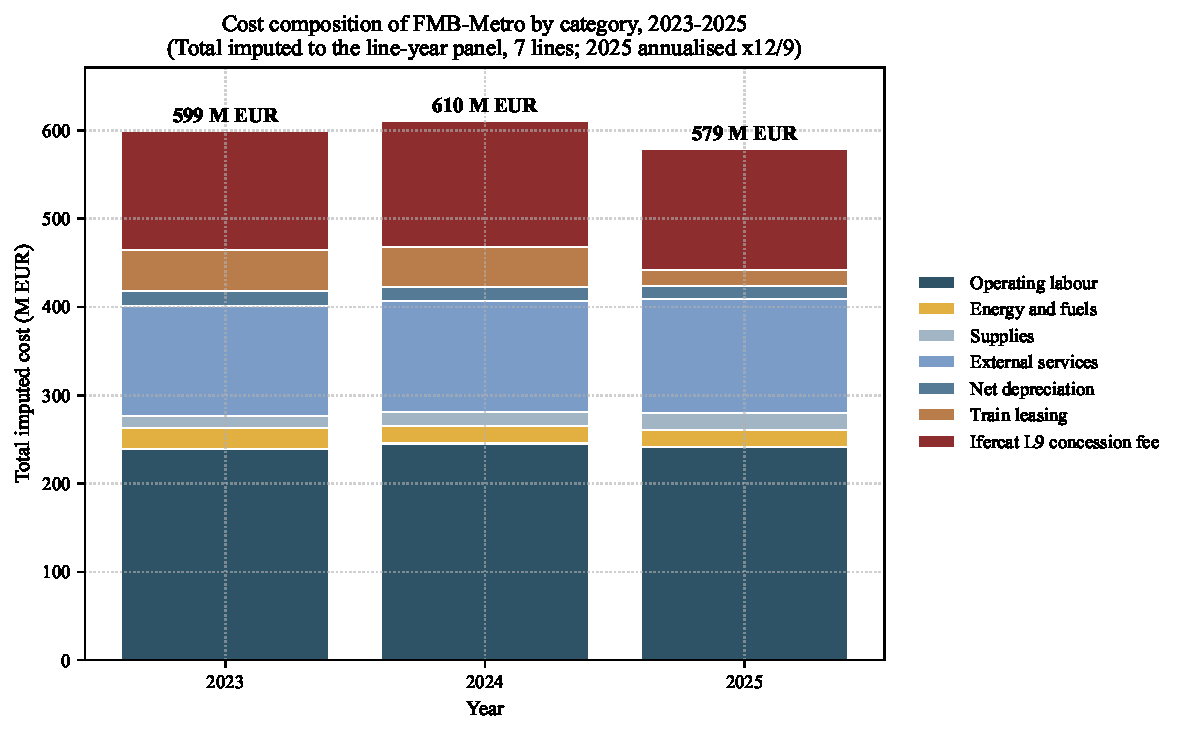
\includegraphics[width=0.74\linewidth]{../outputs/figures/fig1_cost_composition.pdf}
    \caption{Cost composition of FMB-Metro by category and year.}
    \label{fig:cost-comp}
\end{figure}

\subsection{Descriptive statistics}
Table~\ref{tab:descr} summarises the statistics of the line-year panel
($N=21$).

\begin{table}[H]
\centering
\caption{Descriptive statistics of the line-year panel, $N=21$.}
\label{tab:descr}
\footnotesize
\begin{tabular}{lrrrr}
\toprule
Variable & Mean & Std.\ dev. & Min. & Max. \\
\midrule
$C_{\text{total}}$ (M\euro{}) & 84.55 & 24.15 & 50.28 & 124.82 \\
$C_{\text{tec}}$ (M\euro{}) & 60.24 & 26.93 & 26.59 & 109.05 \\
Operating labour (M\euro{}) & 33.79 & 16.25 & 14.94 & 62.81 \\
Energy (M\euro{}) & 2.93 & 1.41 & 1.29 & 5.45 \\
Supplies (M\euro{}) & 2.10 & 1.03 & 0.88 & 4.11 \\
External services (M\euro{}) & 16.24 & 7.85 & 7.29 & 32.30 \\
Net depreciation (M\euro{}) & 2.07 & 0.74 & 1.13 & 3.06 \\
Train leasing (M\euro{}) & 4.80 & 2.29 & 1.15 & 11.65 \\
Ifercat concession fee (M\euro{}) & 18.57 & 35.93 & 0.00 & 84.72 \\
Passengers (M) & 62.55 & 41.42 & 11.04 & 126.39 \\
Imputed car-km (M) & 13.97 & 7.13 & 6.01 & 26.21 \\
$W_L$ (\euro{}/employee) & 60{,}092 & 1{,}166 & 59{,}108 & 61{,}298 \\
$W_E$ (\euro{}/kWh) & 0.0864 & 0.0073 & 0.0815 & 0.0963 \\
\bottomrule
\end{tabular}
\end{table}

% =============================================================================
\section{Calibration strategy}
\label{sec:calib}

\subsection{Calibration vs.\ econometric estimation}
With $N=21$, free estimation of the 17 parameters of the biproduct,
three-input translog is infeasible: the effective degrees of freedom are
low and input prices vary only at the system-year level. We therefore
adopt a strategy of \emph{anchored calibration}, in the methodological
spirit of network regulation \citep{joskow2008,angristpischke2014} and
following the recommendations of \citet{coelli2005} for efficiency
analysis with limited data. First-order parameters are anchored on
observed moments; second-order parameters are anchored on external priors
from the urban rail literature.

\subsection{First-order anchoring}
Mean input shares on total cost are weighted by cost across the 21
observations (equivalent to the aggregate imputed sum). For the
technological cost function $C_{\text{tec}}$:
$\alpha_L = 0.574$, $\alpha_E = 0.050$, $\alpha_O = 0.376$.
First-order cost--output elasticities are anchored on
\citet{savage1997} and \citet{graham2008}: $\beta_1 = 0.45$ and
$\beta_2 = 0.25$.

\subsection{Second-order priors}
Allen--Uzawa elasticities of substitution are taken from
\citet{wheat2015}: $\sigma_{LE}=0.40$, $\sigma_{LO}=0.60$,
$\sigma_{EO}=0.50$. These values are narrow but non-zero, consistent
with substitution operating through limited technological margins
(see Section~\ref{sec:margins}). The $\gamma_{ij}$ are derived from
$\gamma_{ij}=s_i\,s_j(\sigma_{ij}-1)$ and the $\gamma_{ii}$ by
homogeneity. Output--output interactions are
$\delta_{11}=\delta_{22}=0.05$, $\delta_{12}=-0.05$; price--output
interactions are $\rho_{LY_1}=-0.04$, $\rho_{LY_2}=+0.02$,
$\rho_{EY_1}=+0.01$, $\rho_{EY_2}=+0.01$, with $\rho_{OY_k}$ pinned by
homogeneity. The technical trend is $\lambda=-0.005$. The full list of
calibrated values is reported in Table~\ref{tab:params}.

\subsection{Regularity tests}
A well-behaved cost function must satisfy monotonicity in prices and
outputs and concavity in prices. The calibrated technological function
$C_{\text{tec}}$ satisfies \emph{monotonicity in prices} and
\emph{monotonicity in outputs} in all 21 observations and
\emph{approximate concavity} (maximum eigenvalue of the substitution
matrix $M = H + ss' - \text{diag}(s)$ below $10^{-3}$), with a maximum
eigenvalue of $+9.3\times 10^{-5}$ (numerical noise).

\subsection{Treatment of non-technological components}
\label{sec:treatment}

FMB's accounts include two items---the Ifercat L9 concession fee and train
leasing---that do not meet the assumptions underpinning the translog cost
function. A cost function arising from expenditure minimisation must
satisfy Shephard's \citeyearpar{shephard1953} properties (monotonicity,
concavity in prices, linear homogeneity, symmetry), which derive from
duality with a quasi-concave production function and from the operator's
optimisation. The Ifercat fee violates this framework on three
simultaneous grounds: (i) it does not depend on outputs, being a
multi-year contractual payment; (ii) it does not depend on input prices,
being independent of wages or electricity; (iii) it is not an outcome of
optimisation by FMB, which can only accept the fee.

Train leasing admits a softer analogous argument. Rolling stock is a
productive input, but its effective price to FMB is set by long-term
financial-lease contracts with a fixed multi-year payment schedule that
does not respond to year-by-year decisions and cannot be optimised in the
short run. This makes the leasing payment closer to a contractually fixed
transfer than to a variable input price; including it in $C_{\text{tec}}$
would impute optimisation to a payment FMB cannot optimise. We therefore
place it in $F_{\text{inst}}$, a conservative treatment
(Section~\ref{sec:limit}): under an alternative capital-cost modelling,
average cost would shift marginally but marginal cost would remain that of
$C_{\text{tec}}$.

For these reasons we model total cost as an additive decomposition:
\begin{equation}
C_{\text{total}}(Y, W, \text{institutions}) \;=\; C_{\text{tec}}(Y, W) +
F_{\text{inst}},
\label{eq:additive}
\end{equation}
where $C_{\text{tec}}(Y, W)$ is the translog function \eqref{eq:translog},
satisfying the standard properties, and
$F_{\text{inst}} = \text{concession fee} + \text{train leasing}$ is an
additive non-functional component, accounted for but not modelled as
technology. This formulation has precedents in network regulation
\citep{joskow2008} and transport specifically:
\citet{gagnepainivaldi2002} apply an analogous separation in urban bus
concessions, \citet{mizutaniuranishi2013} distinguish infrastructure from
operating costs in Japanese railways, and \citet{wheat2015} warn that
pooling heterogeneous cost components into a single translog distorts the
inferred returns to scale---a logic we extend to institutional
heterogeneity.

As a complementary empirical diagnostic, in Section~\ref{sec:h3} we show
that if $F_{\text{inst}}$ were forced inside the translog specification,
concavity would fail in 10 of 21 observations (48 per cent of the
sample), with a maximum eigenvalue of the Allen--Uzawa substitution
matrix of $+0.0081$. This is the expected microeconomic outcome and
confirms that the additive separation is not optional but theoretically
required.

\subsection{Production technology and substitution margins}
\label{sec:margins}

The cost function in \eqref{eq:translog} is calibrated at the line-year
level. At the train-trip level the technology is essentially Leontief: a
conventional train requires exactly one driver, a fixed electrical
consumption set by the rolling stock, and a fixed maintenance intensity
per car-km---five drivers cannot substitute for one, and a kilowatt-hour
cannot replace a driver \citep{small2007}. Substitution emerges only at
the line-year level, where the operator aggregates many train-trips and
chooses between alternative technologies, vintages and policies. Three
margins are economically relevant and empirically active in FMB during
2023--2025:
\begin{enumerate}[leftmargin=*,topsep=2pt,label=(\alph*)]
\item \textbf{Automation.} L9 and L10 operate driverless under CBTC
signalling, whereas L1--L5 operate with one driver per train. This is a
direct substitution of capital for labour at constant output. The
progressive expansion of L9/L10 service hours over the period reflects
this margin in operation.
\item \textbf{Fleet renewal.} The introduction of series 6000/7000
rolling stock on L1, L3 and L5 reduces electrical consumption per car-km
while delivering the same service. This is energy--capital substitution
at constant output.
\item \textbf{Make-or-buy in maintenance.} The proportion of maintenance
performed in-house versus outsourced to manufacturers (Alstom, CAF,
Siemens) can be adjusted, substituting in-house labour for external
services without altering the output produced.
\end{enumerate}

These margins generate the substitutability the translog captures. They
are narrow---the calibrated Allen--Uzawa elasticities of approximately
0.4--0.6 reflect precisely this narrowness---but non-zero, and sufficient
for the substitution matrix to exhibit the curvature required by Shephard
duality. A fourth potential margin---adjusting service frequency---is not
a clean substitution channel, since it shifts unobserved service quality
(occupancy, waiting time, congestion) rather than substituting factors at
constant output. We adopt the standard convention of treating $Y_2$ as a
proxy that bundles frequency with car-km \citep{farsi2006,daraio2016},
returning to its implications in Section~\ref{sec:limit}.

Crucially, the Ifercat L9 concession fee is impermeable to all three
genuine margins: no automation, fleet-renewal or make-or-buy decision
alters a fee fixed by multi-year contract with the Generalitat. The
concavity failure documented in Section~\ref{sec:h3} is therefore not a
generic departure from cost minimisation but the direct consequence of
forcing into a cost function a component impervious to the only
substitution channels operating in the technology. The additive
decomposition \eqref{eq:additive} formalises this fact: substitutable
components belong inside the cost function and generate concavity;
non-substitutable contractual transfers belong outside it.

% =============================================================================
\section{Results}
\label{sec:resultados}

\subsection{Calibrated parameters of $C_{\text{tec}}$}
Table~\ref{tab:params} reports the calibrated parameters of the
technological cost function $C_{\text{tec}}$.

\begin{table}[H]
\centering
\caption{Calibrated parameters of $C_{\text{tec}}$. The first block
contains first-order parameters (anchor shares and output elasticities);
the second block contains second-order parameters pinned by homogeneity
and the Allen--Uzawa priors.}
\label{tab:params}
\small
\begin{tabular}{lrl}
\toprule
Parameter & $C_{\text{tec}}$ & Source of the prior \\
\midrule
$\alpha_L$  & 0.574 & Data (labour cost share) \\
$\alpha_E$  & 0.050 & Data (energy cost share) \\
$\alpha_O$  & 0.376 & 1 $-\alpha_L-\alpha_E$ \\
$\beta_1$   & 0.45  & Savage 1997, Graham 2008 \\
$\beta_2$   & 0.25  & Savage 1997 \\
$\lambda$   & $-0.005$ & Observed technical trend \\
\midrule
$\gamma_{LL}$ & $+0.1036$ & Homogeneity \\
$\gamma_{EE}$ & $+0.0267$ & Homogeneity \\
$\gamma_{OO}$ & $+0.0957$ & Homogeneity \\
$\gamma_{LE}$ & $-0.0173$ & $\sigma_{LE}=0.40$ (W\&S 2015) \\
$\gamma_{LO}$ & $-0.0863$ & $\sigma_{LO}=0.60$ \\
$\gamma_{EO}$ & $-0.0094$ & $\sigma_{EO}=0.50$ \\
$\delta_{11}$ & $+0.05$ & Modest curvature \\
$\delta_{22}$ & $+0.05$ & Modest curvature \\
$\delta_{12}$ & $-0.05$ & Weakly complementary outputs \\
$\rho_{LY_1}$ & $-0.04$ & Literature prior \\
$\rho_{LY_2}$ & $+0.02$ & Literature prior \\
$\rho_{EY_1}$ & $+0.01$ & Adjusted for frequency rigidity \\
$\rho_{EY_2}$ & $+0.01$ & Literature prior \\
\bottomrule
\end{tabular}
\end{table}

\subsection{H1 --- Density economies}
Under $C_{\text{tec}}$, the passenger-weighted RTD of the system is
$\boldsymbol{2.18}$, comfortably above unity: doubling passengers on the
existing network would reduce technological average cost by approximately
54 per cent. Heterogeneity is marked: lines L1--L5 exhibit RTD in the
range 2.13--2.19, whereas L9/L10 (North and South) reach 2.36--2.43.
The reason is that the automated lines operate with a rigid frequency
and low occupancy, so each additional passenger absorbs idle capacity.

\begin{figure}[H]
    \centering
    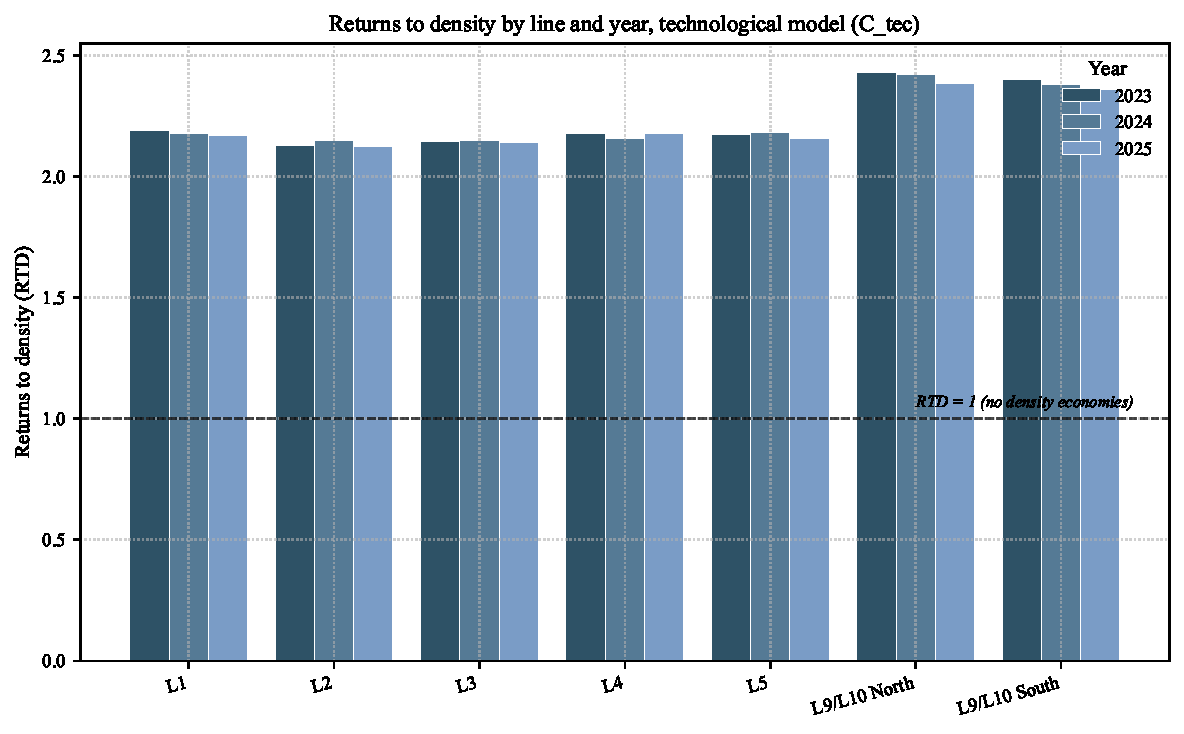
\includegraphics[width=0.72\linewidth]{../outputs/figures/fig2_rtd_by_line.pdf}
    \caption{Returns to density by line-year, technological cost function
    $C_{\text{tec}}$.}
    \label{fig:rtd}
\end{figure}

\subsection{H2 --- Marginal vs.\ average cost}
The passenger-weighted technological average cost of the system is
0.915~\euro{}/pax; the corresponding marginal cost is 0.417~\euro{}/pax.
The MC/AC ratio is $\boldsymbol{0.46}$, implying a Boiteux optimal
subsidy of $\boldsymbol{54.5}$ per cent of technological average cost.
Figure~\ref{fig:mc-ac} reports the line averages (left) and the temporal
evolution (right); the Boiteux optimal subsidy is stable across the three
years.

\begin{figure}[H]
    \centering
    \begin{subfigure}{0.53\linewidth}
        \centering
        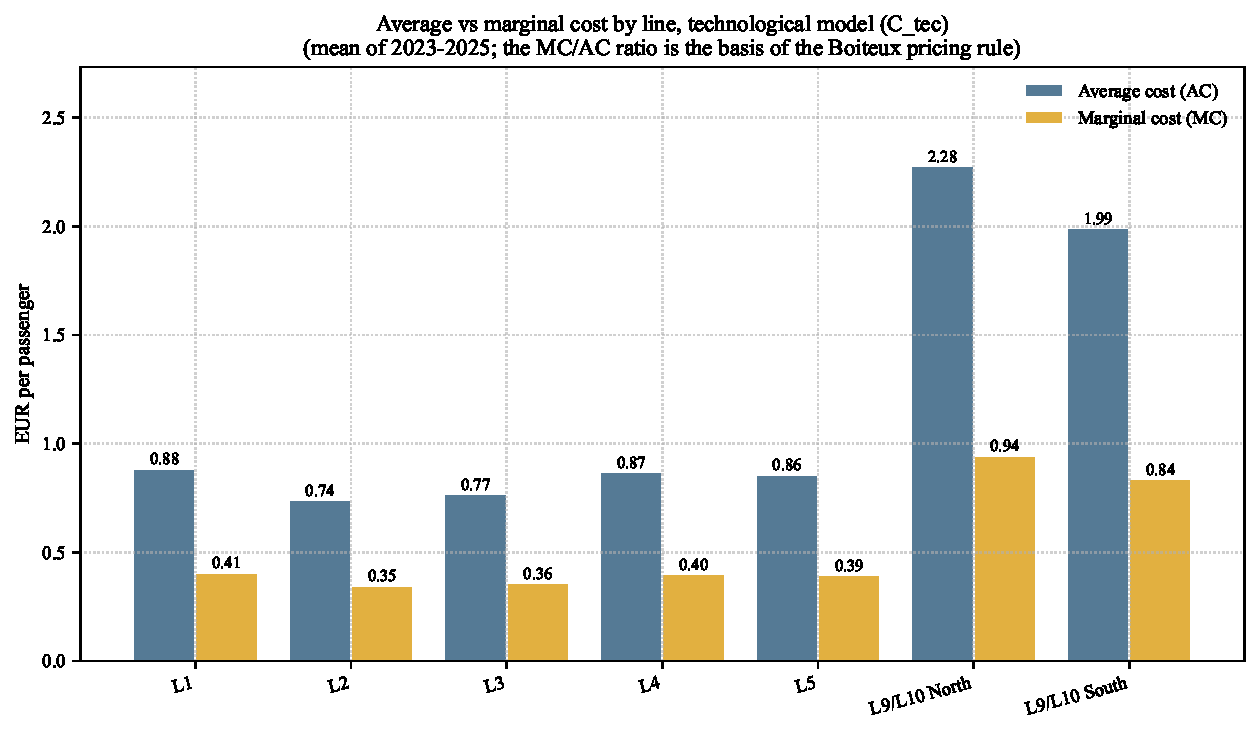
\includegraphics[width=\linewidth]{../outputs/figures/fig3_mc_vs_ac.pdf}
        \caption{AC vs.\ MC by line, 2023--2025 mean.}
        \label{fig:mc-ac-a}
    \end{subfigure}\hfill
    \begin{subfigure}{0.45\linewidth}
        \centering
        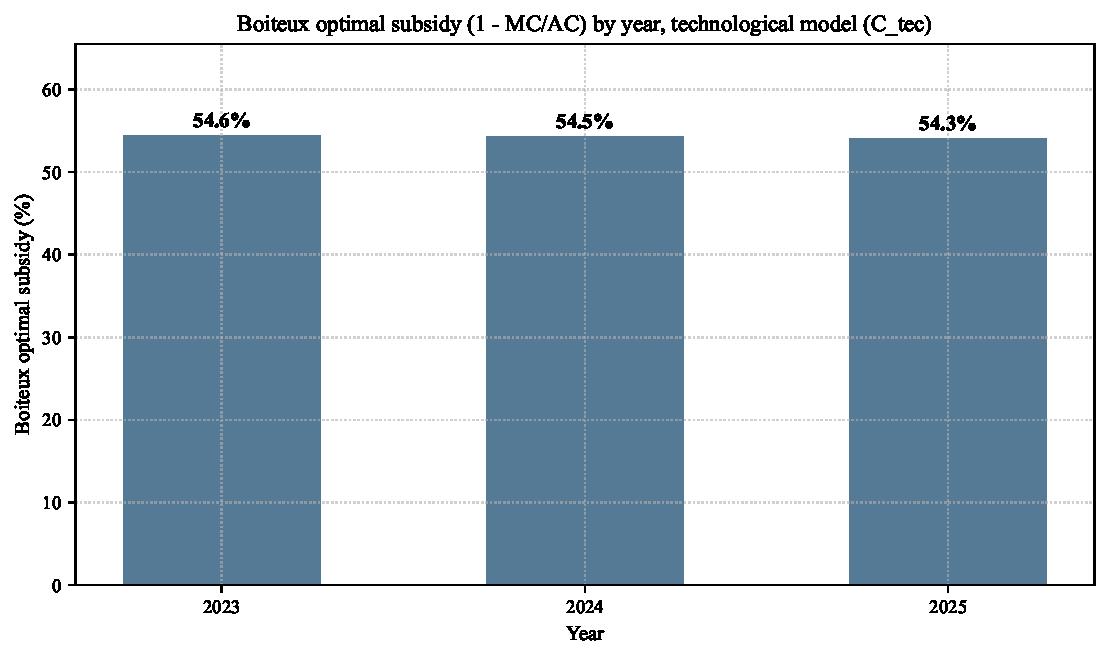
\includegraphics[width=\linewidth]{../outputs/figures/fig4_subsidy_boiteux.pdf}
        \caption{Boiteux optimal subsidy by year.}
        \label{fig:subsidy}
    \end{subfigure}
    \caption{Average vs.\ marginal cost and the implied Boiteux optimal
    subsidy, technological cost function $C_{\text{tec}}$.}
    \label{fig:mc-ac}
\end{figure}

\subsection{H3 --- Technology vs.\ institutional decomposition}
\label{sec:h3}

\subsubsection*{(a) Magnitude and composition of $F_{\text{inst}}$}
$F_{\text{inst}}$ accounts for approximately 29 per cent of total
declared cost. Under the calibrated parameters this corresponds to about
0.38~\euro{} per passenger system-wide, on top of the technological
average cost of 0.91~\euro{} per passenger. Table~\ref{tab:h3} summarises
the closing decomposition.

\begin{table}[H]
\centering
\caption{H3 closing decomposition: $C_{\text{total}} = C_{\text{tec}} +
F_{\text{inst}}$. Aggregates use passenger-weighted means over the panel.}
\label{tab:h3}
\footnotesize
\begin{tabularx}{\linewidth}{l c c c}
\toprule
Metric & $C_{\text{tec}}$ (technological) & $F_{\text{inst}}$ (institutional) & $C_{\text{total}}$ (full) \\
\midrule
Mean AC (\euro{}/pax) & 0.91 & 0.38 & 1.29 \\
Mean MC (\euro{}/pax) & 0.42 & 0.00 & 0.42 \\
Returns to density (RTD) & 2.18 & N/A (fixed) & N/A \\
Cost share & 71\% & 29\% & 100\% \\
Satisfies Shephard's properties & Yes & Not applicable (non-technological) & No (concavity fails in 10/21 obs.) \\
\bottomrule
\end{tabularx}
\end{table}

$F_{\text{inst}}$ is overwhelmingly concentrated in L9/L10: those two
lines absorb 82 per cent of the institutional component, and for them
$F_{\text{inst}}$ represents 70 per cent of total declared cost. By
contrast, $F_{\text{inst}}$ is only 8 per cent of total cost in lines
L1--L5. This concentration is a direct consequence of how the concession
fee is allocated by construction (100 per cent to L9/L10 by the Ifercat
contract); the train-leasing component is more evenly spread.

\begin{figure}[H]
    \centering
    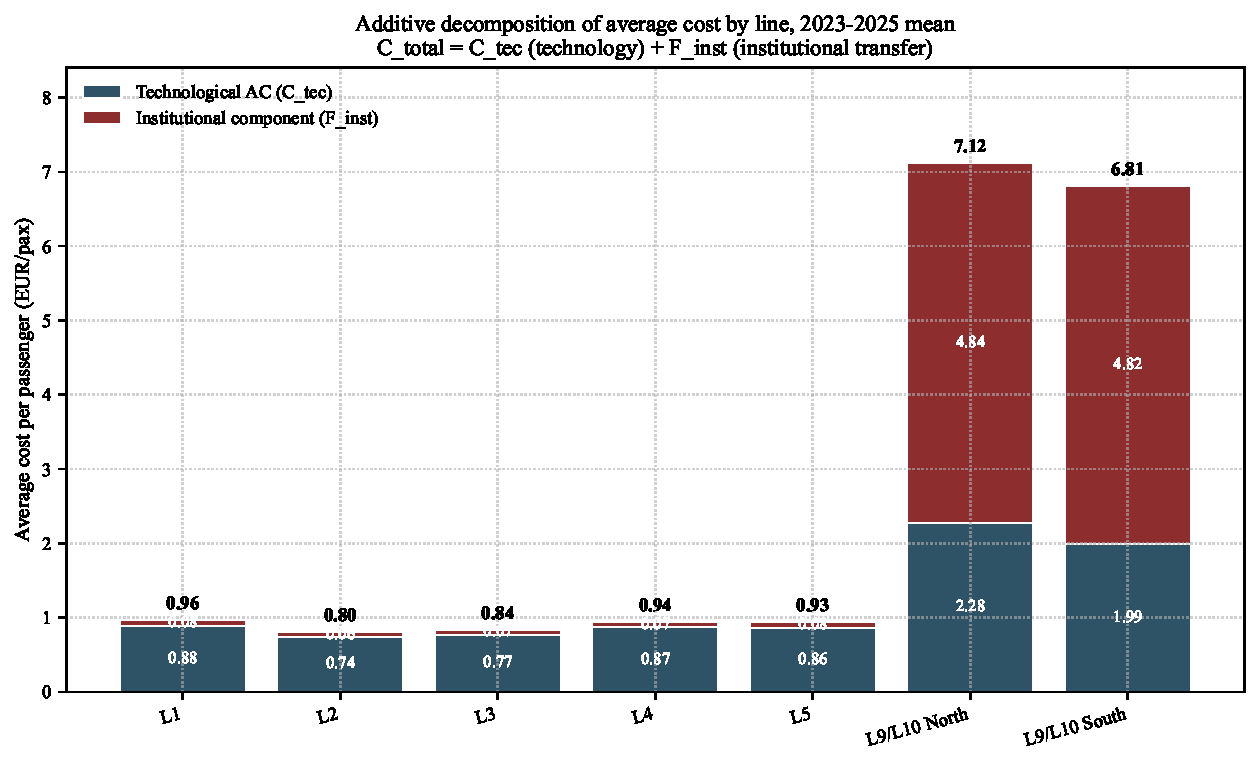
\includegraphics[width=0.78\linewidth]{../outputs/figures/fig_additive_decomposition.pdf}
    \caption{Additive decomposition of average cost by line, 2023--2025
    mean. The dark band is technological average cost ($C_{\text{tec}}$);
    the red band is the institutional component ($F_{\text{inst}}$). The
    visible total is $C_{\text{total}}$.}
    \label{fig:add-decomp}
\end{figure}

\subsubsection*{(b) Convergent technological cost across lines}
Across the seven blocks the technological average cost is concentrated in
a narrow range, approximately 0.7--1.0~\euro{} per passenger. Total
declared average cost in L9/L10 reaches 6--8~\euro{} per passenger. The
gap between the two figures is entirely accounted for by
$F_{\text{inst}}$, not by operational inefficiency. Once the institutional
component is removed, the lines look technologically similar; the
divergence reappears only when the concession fee is included.

\subsubsection*{(c) Concavity diagnostic}
Forcing $F_{\text{inst}}$ inside the translog specification breaks
Shephard concavity. Figure~\ref{fig:conc-diag} reports the maximum
eigenvalue of the Allen--Uzawa substitution matrix for each of the 21
line-year observations: 10 observations (48 per cent) yield a positive
eigenvalue, with a maximum of $+0.0081$, concentrated in L9/L10 where
the fee weighs most heavily on the cost share.

\begin{figure}[H]
    \centering
    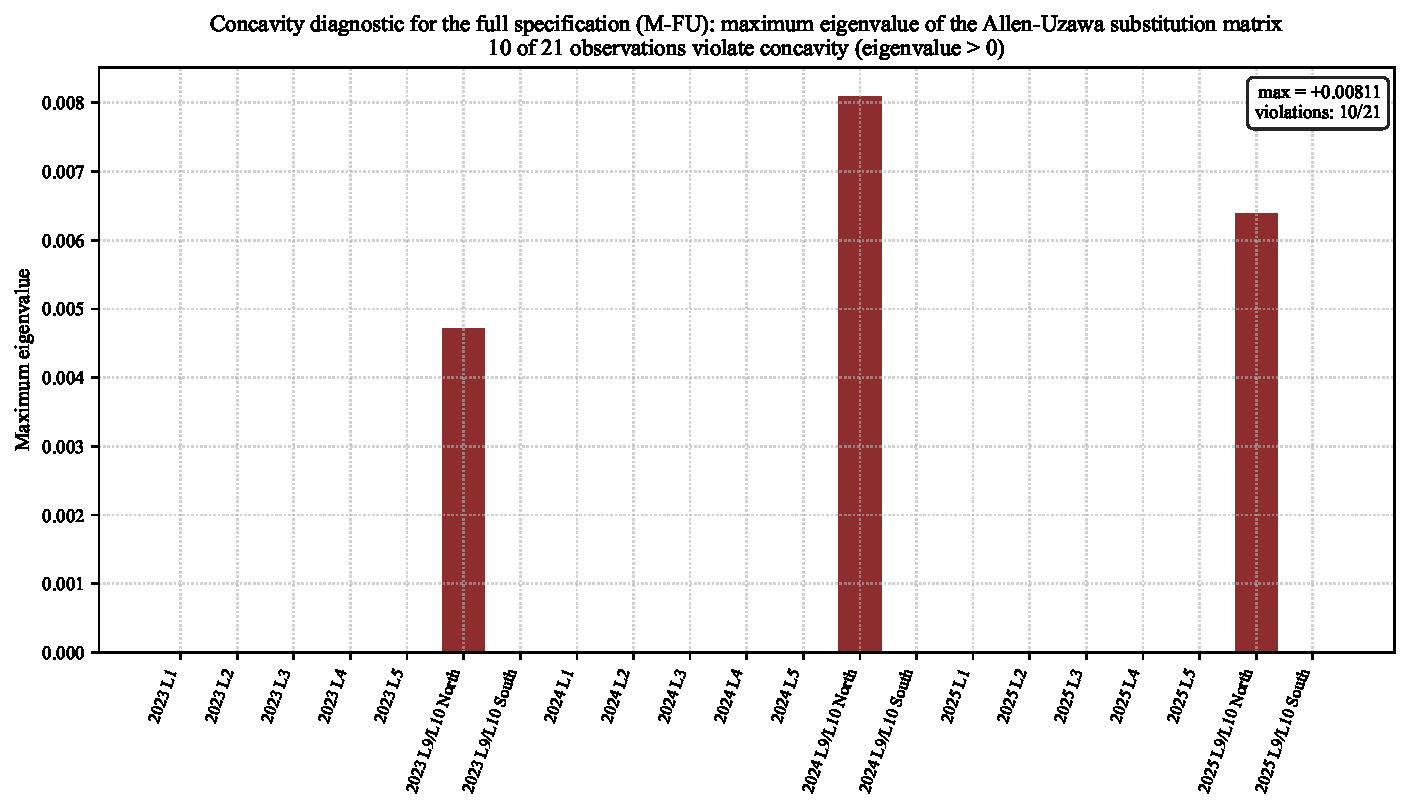
\includegraphics[width=0.82\linewidth]{../outputs/figures/fig_concavity_diagnostic.pdf}
    \caption{Concavity diagnostic for the full specification: maximum
    eigenvalue of the Allen--Uzawa substitution matrix, by line-year.
    Observations with eigenvalue $>0$ violate Shephard concavity.}
    \label{fig:conc-diag}
\end{figure}

This failure is the expected microeconomic result. As argued in
Section~\ref{sec:margins}, the concession fee is impermeable to the three
substitution margins (automation, fleet renewal, maintenance make-or-buy)
that generate the concavity property in the technological cost function.
A function that includes $F_{\text{inst}}$ is asked to represent as
technology something that is not technology, and the substitution matrix
loses the required curvature precisely where this contradiction is most
binding. Forcing $F_{\text{inst}}$ inside the translog also produces a
MAPE of 53 per cent, compared with 14 per cent for $C_{\text{tec}}$---a
3.8$\times$ degradation. This empirically confirms the methodological
decision made in Section~\ref{sec:treatment}.

\subsection{H4 --- Heterogeneity L9/L10 vs.\ L1--L5}
Figure~\ref{fig:hetero} illustrates the gap in average cost between the
conventional lines (L1--L5) and the automated lines (L9/L10). Under
$C_{\text{tec}}$ alone the difference is bounded: the technology of the
two groups is comparable in average cost per passenger, with automation
shifting the labour share down without altering the order of magnitude
of total operating cost per passenger. Under $C_{\text{total}}$ the gap
widens dramatically because $F_{\text{inst}}$, concentrated on L9/L10,
adds several euros per passenger on the institutional side. The
implication is that any operational efficiency gain from automation is
swamped by the concession fee in the consolidated accounts---an
empirical fact that has nothing to do with the technology of driverless
operation as such.

Figure~\ref{fig:hetero} (right) reports the operating cost shares by
year, which remain stable around a labour-dominated structure (57--58
per cent), with energy at 4.6--5.9 per cent.

\begin{figure}[H]
    \centering
    \begin{subfigure}{0.52\linewidth}
        \centering
        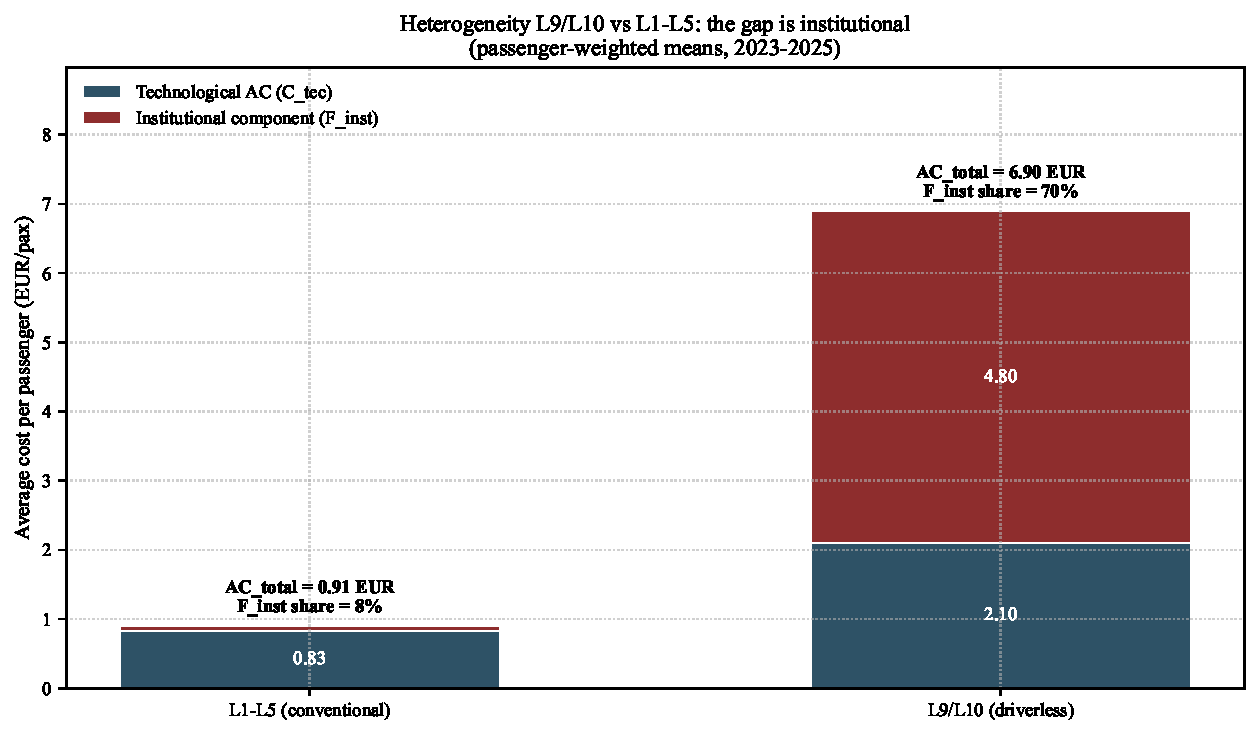
\includegraphics[width=\linewidth]{../outputs/figures/fig6_heterogeneity_L9.pdf}
        \caption{L9/L10 vs.\ L1--L5: the gap is institutional.}
        \label{fig:hetero-a}
    \end{subfigure}\hfill
    \begin{subfigure}{0.46\linewidth}
        \centering
        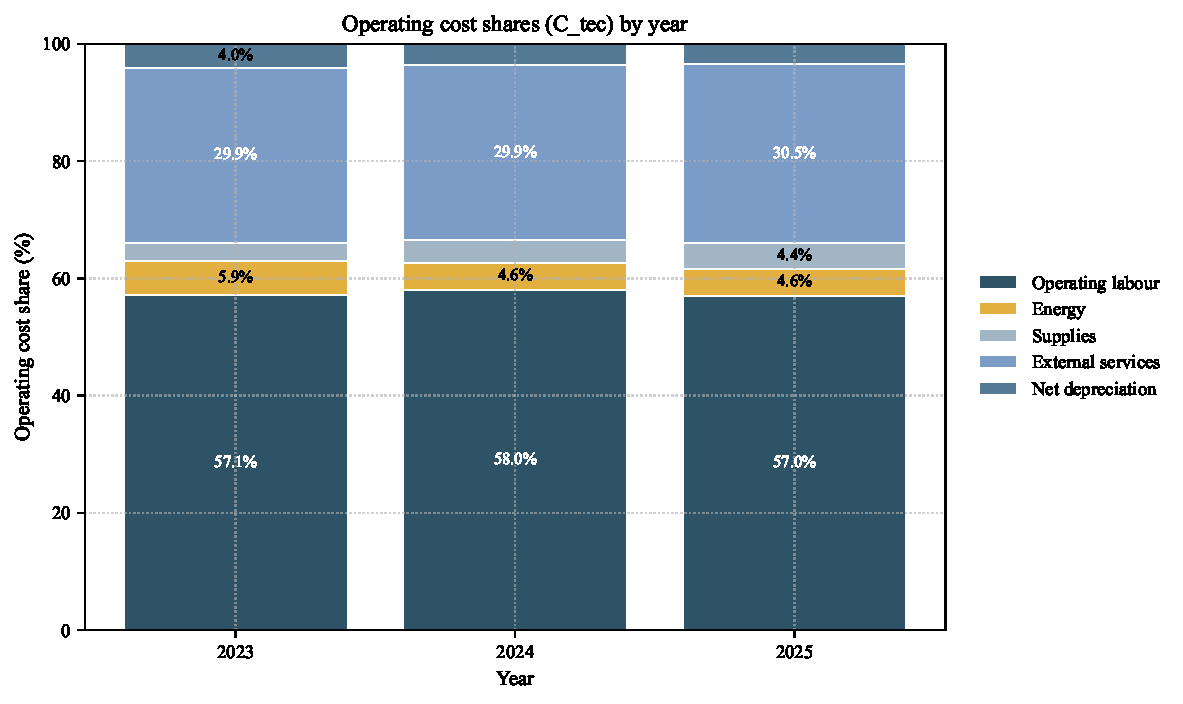
\includegraphics[width=\linewidth]{../outputs/figures/fig5_cost_shares_operating.pdf}
        \caption{Operating cost shares ($C_{\text{tec}}$) by year.}
        \label{fig:shares}
    \end{subfigure}
    \caption{Heterogeneity and operating cost shares. Left: stacked bars
    decompose the passenger-weighted average cost into $C_{\text{tec}}$
    (technological) and $F_{\text{inst}}$ (institutional). Right: stable
    labour-dominated cost structure of $C_{\text{tec}}$.}
    \label{fig:hetero}
\end{figure}

% =============================================================================
\section{Robustness}
\label{sec:robustez}

\subsection{Accounting validation}
The ratio of predicted to observed cost by line-year has a mean absolute
percentage error (MAPE) of 14.1 per cent under $C_{\text{tec}}$. As
discussed in Section~\ref{sec:h3}, forcing $F_{\text{inst}}$ inside the
translog raises the MAPE to 52.9 per cent. The difference is the
signature of the additive decomposition, not noise.

\subsection{Sensitivity to priors}
Figure~\ref{fig:tornado} reports the sensitivity of RTD to the priors.
The Allen--Uzawa elasticities $\sigma$ and the time trend $\lambda$ do
not materially affect RTD (the $\gamma_{ij}$ terms enter only at second
order and cancel at the sample mean). The $\beta_1$ prior does affect
RTD by construction: it is the direct anchor. Varying $\beta_1$ by
$\pm 0.10$ shifts RTD between 1.79 and 2.79.

\begin{figure}[H]
    \centering
    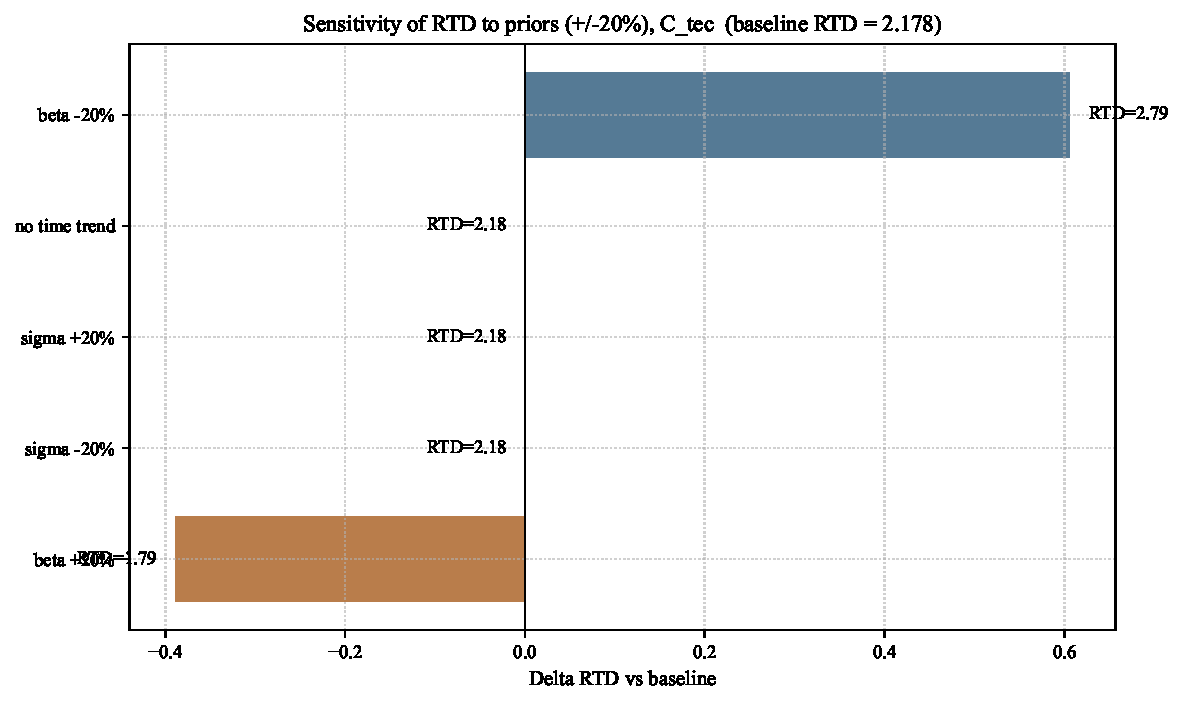
\includegraphics[width=0.8\linewidth]{../outputs/figures/fig7_tornado.pdf}
    \caption{Sensitivity of RTD to priors (tornado plot), $C_{\text{tec}}$.}
    \label{fig:tornado}
\end{figure}

\subsection{Alternative imputation by passengers}
Redistributing all costs proportionally to passengers and re-estimating
$\beta$ by ordinary least squares on the re-imputed panel yields
$\beta_1 = 1.000$ and $\beta_2 = 0.000$ exactly: $\text{RTD} = 1$. This
is mechanical---imputation defines the elasticity---and demonstrates
that the use of car-km as the imputation key is a \emph{condition for
identification}. The native OLS estimate by car-km imputation yields
RTD~$=-42.6$, confirming that the free regression is uninformative with
this variability. Anchoring $\beta$ on the literature is therefore
indispensable.

\subsection{Aggregate $T=3$ model}
Abandoning the line-year panel and attempting to solve $T=3$ by finite
differences year on year---two equations in two unknowns $\beta_1,
\beta_2$ with $\lambda=0$---yields a variability matrix $X$ with
condition number $\mathbf{30.5}$ and parameter estimates of $\beta_1
=+0.008$ and RTD $=+129.9$. The aggregate model is structurally
ill-identified.

\subsection{Monoproduct specification}
Omitting $Y_2$ and calibrating with $\beta_1 = 0.70$ (the sum of the
biproduct $\beta$'s) yields a passenger-weighted RTD of 1.38, against
2.18 under the biproduct $C_{\text{tec}}$. The biproduct specification
is therefore essential: the supplied network and realised demand are
economically distinct outputs, and the monoproduct version
under-estimates density economies.

\subsection{Excluding 2025}
Recalibrating using only 2023--2024 ($N=14$), the input cost shares
change by $+0.19$~pp ($s_L$), and the RTD remains within $\pm 10^{-3}$.
Inclusion of the annualised 2025 data does not distort the calibration.

\medskip
Taken together, the robustness analyses confirm that the central findings
(RTD~$\approx 2.18$, MC/AC~$\approx 0.46$, and $F_{\text{inst}}$ at some 29
per cent of total declared cost with zero contribution to marginal cost)
do not depend on the imputation key, on the partial 2025 observations, or
on the specific priors. They do depend on the additive separation between
$C_{\text{tec}}$ and $F_{\text{inst}}$, defended theoretically in
Sections~\ref{sec:treatment}--\ref{sec:margins} and empirically in
Section~\ref{sec:h3}.

% =============================================================================
\section{Discussion and policy implications}
\label{sec:politica}

\subsection{Closing argument on H3}
Three results, taken together, frame the central regulatory message of
this paper. \emph{(i)} The institutional component $F_{\text{inst}}$
represents around 29 per cent of FMB's total declared cost, larger than
the entire energy bill and second only to operating labour. \emph{(ii)}
The concavity failure of the translog specification when $F_{\text{inst}}$
is forced inside it formally demonstrates that the concession fee is not
technological cost in any sense compatible with the dual structure of
cost minimisation. \emph{(iii)} Any assessment of FMB's operational
efficiency, or any social cost--benefit analysis of L9/L10, that does
not separate $C_{\text{tec}}$ from $F_{\text{inst}}$ is biased by
construction.

\subsection{Anchoring in the European regulatory framework}
Directive 2012/34/EU \citep{directive2012} mandates accounting separation
between infrastructure managers and operators, on the rationale that
mixing infrastructure-access charges with operating costs distorts
efficiency signals and biases regulatory comparisons. Urban metro systems
fall outside its formal scope, but the logic applies with greater force to
FMB, where the Ifercat fee---nearly a quarter of total declared cost,
larger than the entire energy bill---is paid to a separate public entity
that owns the infrastructure yet appears as a current operating expense
in consolidated accounts. The microeconomic demonstration of this
paper---that $F_{\text{inst}}$ cannot be represented within a cost
function with standard properties---provides the formal foundation for
what the directive prescribes on regulatory grounds: $F_{\text{inst}}$
must be reported separately for efficiency assessments to be meaningful,
regardless of whether formal compliance is required.

\subsection{Policy recommendations}

\paragraph{Accounting separation aligned with Directive 2012/34/EU.}
Presenting the Ifercat fee as a current operating expense alongside labour
and energy is not innocuous: it mixes a contractual infrastructure
transfer with technological inputs, biasing operating-efficiency
indicators and any benchmarking against peer metros. The minimal
recommendation is to report the fee separately, so that downstream users
can recover the technological cost function and assess efficiency on a
clean basis.

\paragraph{Reform of the fee: a capacity charge rather than a fixed
multi-year fee.} The current fee is largely independent of effective use
of L9/L10 capacity. Replacing it, in whole or in part, with a charge
indexed to car-km or train-paths delivered would align the operator's
perceived cost with actual infrastructure utilisation, generating
efficiency signals consistent with network regulation
\citep{joskow2008,gomezlobo2014}; a hybrid fixed-plus-variable scheme is a
natural intermediate. Relatedly, the underlying infrastructure has an
expected useful life above 75 years, yet the schedule front-loads cost
recovery, pressuring FMB's annual P\&L; reprofiling it closer to the asset
life would reduce the $F_{\text{inst}}$ share in current cost without
altering the consolidated public-debt position.

\paragraph{Train leasing and lessons for other cities.} Leasing delivers
dynamic efficiency (quicker fleet renewal, risk-sharing) at the static
cost of a rigid recurrent expense; greater transparency on the split
between capital recovery and service would inform the regulatory debate.
More broadly, any urban system financing infrastructure through off-budget
debt repaid via long-term availability fees inherits the same difficulty
as L9/L10: the Ifercat architecture is efficient on the financing side but
consequential for the interpretation of operating cost.

\subsection{Qualitative comparison with European peers}
Madrid Metro operates under a different institutional architecture: the
infrastructure is fully publicly owned and there is no analogous
infrastructure-access fee in the operator's accounts. RATP Paris
integrates infrastructure ownership and operation under a single public
entity, so that infrastructure recovery is internal to the same balance
sheet. Transport for London (TfL) operates under concession contracts
with explicit accounting separation between infrastructure managers and
operators. Among major European systems, only Barcelona's L9/L10
combines this Ifercat-style concession fee with consolidated operator
accounts that present the fee as a current operating expense---hence
the regulatory peculiarity of the Barcelona case.

% =============================================================================
\section{Limitations}
\label{sec:limit}

\begin{itemize}[leftmargin=*,topsep=2pt]
\item \textbf{Sample size.} $N=21$ is insufficient for classical
econometric estimation. The anchored calibration is a systematic
response, not a methodological excuse.
\item \textbf{Cost imputation.} The line-level allocation is derived,
not accounting. The sensitivity to the imputation key
(Section~\ref{sec:robustez}) bounds the issue, but does not eliminate
it as a source of error.
\item \textbf{Calibration is not causal identification.} The priors are
informed choices, not estimates. Material changes in $\beta_1$ shift
RTD proportionally.
\item \textbf{Over-parametrised translog.} A free translog would have
17 parameters for 21 observations; calibration brings the effective
degrees of freedom down to 4--5.
\item \textbf{Annualised 2025.} The $\times 12/9$ rescaling may
incorporate seasonality. The robustness check on excluding 2025 shows
that this is immaterial for the cost shares.
\item \textbf{Heterogeneity not observed.} \citet{farsi2006} shows that
ignoring line fixed effects can bias the elasticities. Our calibration
absorbs part of this through line-specific $\alpha_O$ adjustments, but
a structured fixed-effects analysis remains pending.
\item \textbf{Conservative treatment of train leasing.} The treatment of
train leasing as purely institutional is conservative. If it were
modelled as capital with linear depreciation, AC would change
marginally but MC would remain that of $C_{\text{tec}}$, because capital
cost is fixed in the short run.
\item \textbf{No interaction in the additive decomposition.} The
decomposition assumes no interaction between $F_{\text{inst}}$ and
$C_{\text{tec}}$. This is reasonable since the concession fee is
independent of operational decisions, but a finer analysis with internal
TMB accounting data could detect second-order interactions.
\item \textbf{Variable-cost alternatives.} Variable-cost models with
quasi-fixed inputs \citep{cavesswanson1981} could in principle apply,
but require long time series for partial-adjustment identification.
With $T=3$, the additive decomposition is the only viable identification
strategy that preserves microeconomic properties.
\item \textbf{Service quality.} Frequency, waiting time, occupancy and
reliability are product dimensions the operator can adjust with inputs;
our model implicitly assumes quality moves proportionally with car-km
($Y_2$), so the reported returns to density should be read as conditional
on approximately constant service quality. As argued in
Section~\ref{sec:margins}, this does not affect the central conclusion on
$F_{\text{inst}}$: the concession fee is impermeable to all three genuine
substitution margins, so its exclusion from $C_{\text{tec}}$ is required
by the technology, not by the constant-quality assumption.
\item \textbf{Temporal pattern of $F_{\text{inst}}$.} The $F_{\text{inst}}$
share falls from 30.2 (2023) and 30.7 (2024) to 26.8 per cent in the 2025
annualised figures. We cannot distinguish genuine reductions in the
fee/leasing from faster growth in $C_{\text{tec}}$ or artefacts of the
$\times 12/9$ annualisation; the conclusions on density and the additive
decomposition are unaffected, holding uniformly across years.
\end{itemize}

% =============================================================================
\section{Conclusions}
\label{sec:concl}

We have calibrated a multiproduct translog cost function for FMB-TMB on
a line-year panel of 21 observations. The function satisfies the
regularity tests when restricted to its technological component
$C_{\text{tec}}$, and it leaves a formal trace of the distortion induced
by the Ifercat L9 concession fee when the latter is forced inside the
translog. Returns to density are substantial (RTD~$\approx 2.18$),
marginal cost is roughly half of average cost (Boiteux optimal subsidy
of approximately 54 per cent), and the institutional component
$F_{\text{inst}}$ accounts for around 29 per cent of total declared
cost. The methodological contribution is the formal separation, on
microeconomic grounds, of the technological cost function from the
quasi-fixed contractual transfers that share the FMB consolidated
accounts with it. The policy contribution is to align the empirical
treatment of the Ifercat concession fee with the accounting-separation
principle of Directive 2012/34/EU for the broader rail sector.

% =============================================================================
\bibliography{paper_translog_fmb}
% Manual bibliography:
{\small
\begin{thebibliography}{99}

\bibitem[Allais(1947)]{allais1947}
Allais, M.\ (1947).
\textit{Le probl\`{e}me de la coordination des transports et la th\'{e}orie
\'{e}conomique.}
Bulletin des Ponts et Chauss\'{e}es et des Mines.

\bibitem[Angrist and Pischke(2014)]{angristpischke2014}
Angrist, J.~D.\ and Pischke, J.-S.\ (2014).
\textit{Mastering Metrics: The Path from Cause to Effect.}
Princeton University Press.

\bibitem[Boiteux(1956)]{boiteux1956}
Boiteux, M.\ (1956).
Sur la gestion des monopoles publics astreints \`{a} l'\'{e}quilibre
budg\'{e}taire.
\textit{Econometrica}, 24(1), 22--40.

\bibitem[Cantos et al.(2010)]{cantos2010}
Cantos, P., Pastor, J.~M.\ and Serrano, L.\ (2010).
Vertical and horizontal separation in the European railway sector and
its effects on productivity.
\textit{Journal of Transport Economics and Policy}, 44(2), 139--160.

\bibitem[Caves et al.(1984)]{caves1984}
Caves, D.~W., Christensen, L.~R.\ and Tretheway, M.~W.\ (1984).
Economies of density vs.\ economies of scale.
\textit{RAND Journal of Economics}, 15(4), 471--489.

\bibitem[Caves et al.(1981)]{cavesswanson1981}
Caves, D.~W., Christensen, L.~R.\ and Swanson, J.~A.\ (1981).
Productivity growth, scale economies, and capacity utilization in U.S.\
railroads, 1955--74.
\textit{American Economic Review}, 71(5), 994--1002.

\bibitem[Christensen et al.(1973)]{cjl1973}
Christensen, L.~R., Jorgenson, D.~W.\ and Lau, L.~J.\ (1973).
Transcendental logarithmic production frontiers.
\textit{Review of Economics and Statistics}, 55(1), 28--45.

\bibitem[Coelli et al.(2005)]{coelli2005}
Coelli, T., Rao, D., O'Donnell, C.\ and Battese, G.\ (2005).
\textit{An Introduction to Efficiency and Productivity Analysis.}
2nd ed.\ Springer.

\bibitem[Daraio et al.(2016)]{daraio2016}
Daraio, C., Diana, M., Di Costa, F., Leporelli, C., Matteucci, P.\ and
Nastasi, A.\ (2016).
Efficiency and effectiveness in the urban public transport sector: a
critical review with directions for future research.
\textit{European Journal of Operational Research}, 248(1), 1--20.

\bibitem[De Borger and Kerstens(2000)]{debergerkerstens2000}
De Borger, B.\ and Kerstens, K.\ (2000).
The performance of bus-transit operators.
In \textit{Handbook of Transport Modelling}, Pergamon, 577--595.

\bibitem[Diewert(1971)]{diewert1971}
Diewert, W.~E.\ (1971).
An application of the Shephard duality theorem: a generalized Leontief
production function.
\textit{Journal of Political Economy}, 79(3), 481--507.

\bibitem[Directive 2012/34/EU(2012)]{directive2012}
Directive 2012/34/EU of the European Parliament and of the Council of
21~November~2012 establishing a single European railway area.
\textit{Official Journal of the European Union}, L~343, 14.12.2012,
pp.~32--77.

\bibitem[Farsi et al.(2006)]{farsi2006}
Farsi, M., Filippini, M.\ and Kuenzle, M.\ (2006).
Cost efficiency in regional bus companies: an application of
alternative stochastic frontier models.
\textit{Journal of Transport Economics and Policy}, 40(1), 95--118.

\bibitem[Gagnepain and Ivaldi(2002)]{gagnepainivaldi2002}
Gagnepain, P.\ and Ivaldi, M.\ (2002).
Incentive regulatory policies: the case of public transit systems in
France.
\textit{RAND Journal of Economics}, 33(4), 605--629.

\bibitem[G\'omez-Lobo and Briones(2014)]{gomezlobo2014}
G\'omez-Lobo, A.\ and Briones, J.\ (2014).
Incentives in bus concession contracts: a review of several experiences
in Latin America.
\textit{Transport Reviews}, 34(2), 246--265.

\bibitem[Graham(2008)]{graham2008}
Graham, D.~J.\ (2008).
Productivity and efficiency in urban railways: parametric and
non-parametric estimates.
\textit{Transportation Research Part E}, 44(1), 84--99.

\bibitem[Joskow(2008)]{joskow2008}
Joskow, P.~L.\ (2008).
Incentive regulation and its application to electricity networks.
\textit{Review of Network Economics}, 7(4), 547--560.

\bibitem[Matas and Raymond(2009)]{matasraymond2009}
Matas, A.\ and Raymond, J.~L.\ (2009).
Costes y eficiencia del transporte p\'ublico urbano en Espa\~na.
\textit{IEB Working Paper} 2009/19.

\bibitem[Mizutani and Uranishi(2013)]{mizutaniuranishi2013}
Mizutani, F.\ and Uranishi, S.\ (2013).
Does vertical separation reduce cost? An empirical analysis of the rail
industry in European and East Asian OECD countries.
\textit{Journal of Regulatory Economics}, 43(1), 31--59.

\bibitem[Nash and Preston(1995)]{nashpreston1995}
Nash, C.~A.\ and Preston, J.~M.\ (1995).
Railway costing: theory and practice.
\textit{International Journal of Transport Economics}, 22(2), 153--170.

\bibitem[Pigou(1920)]{pigou1920}
Pigou, A.~C.\ (1920).
\textit{The Economics of Welfare.} Macmillan.

\bibitem[Savage(1997)]{savage1997}
Savage, I.\ (1997).
Scale economies in U.S.\ rail transit systems.
\textit{Transportation Research Part A}, 31(6), 459--473.

\bibitem[Shephard(1953)]{shephard1953}
Shephard, R.~W.\ (1953).
\textit{Cost and Production Functions.} Princeton University Press.

\bibitem[Small and Verhoef(2007)]{small2007}
Small, K.~A.\ and Verhoef, E.~T.\ (2007).
\textit{The Economics of Urban Transportation.} 2nd ed.\ Routledge.

\bibitem[Uzawa(1962)]{uzawa1962}
Uzawa, H.\ (1962).
Production functions with constant elasticities of substitution.
\textit{Review of Economic Studies}, 29(4), 291--299.

\bibitem[Wheat and Smith(2015)]{wheat2015}
Wheat, P.\ and Smith, A.~S.~J.\ (2015).
Do the usual results of railway returns to scale and density vary with
scope?
\textit{Transport Reviews}, 35(3), 263--286.

\end{thebibliography}
}

% =============================================================================
\appendix

\section{Derivation of RTD and marginal cost}
\label{app:derivation}

From the translog cost function \eqref{eq:translog}, the cost--passenger
elasticity at a given observation (with centred variables $w_L, w_E,
y_1, y_2$) is
\begin{equation}
\varepsilon_{Y_1} \;=\; \frac{\partial \ln C}{\partial \ln Y_1}
\;=\; \beta_1 + \delta_{11}\, y_1 + \delta_{12}\, y_2
       + \rho_{LY_1}\, w_L + \rho_{EY_1}\, w_E .
\end{equation}
The marginal cost per passenger is
$\text{MC} = \partial C / \partial Y_1 = \varepsilon_{Y_1}\, C / Y_1$,
average cost is $\text{AC} = C / Y_1$, and hence
$\text{MC}/\text{AC} = \varepsilon_{Y_1}$.
RTD is the reciprocal: $\text{RTD} = 1/\varepsilon_{Y_1}$. At the sample
mean (all centred variables zero), $\varepsilon_{Y_1} = \beta_1$.

The predicted input cost share (Shephard) is
\begin{equation}
s_i \;=\; \alpha_i + \sum_j \gamma_{ij}\, w_j + \sum_k \rho_{ik}\, y_k.
\end{equation}
Concavity in prices is equivalent to negative semi-definiteness of the
substitution matrix
$M_{ij} = \gamma_{ij} + s_i s_j - \delta_{ij}^K\, s_i$, where
$\delta_{ij}^K$ is the Kronecker delta.

\section{Detailed imputation keys}
\label{app:keys}

\subsection{Car-km share (\emph{share\_ckm})}
$\text{share\_ckm}_{l,t} = \dfrac{\text{peak\_trains}_{l,t}\times
\text{km\_line}_l}{\sum_{l'} \text{peak\_trains}_{l',t}\times
\text{km\_line}_{l'}}$,
with the denominator aggregated over all lines (including L11 and the
Funicular). In 2024:
\begin{center}
\footnotesize
\begin{tabular}{lrrrr}
\toprule
Line & peak trains & km of line & trains$\cdot$km & share \\
\midrule
L1   & 34 & 22.4 &   761.6 & 25.55\% \\
L2   & 20 & 13.1 &   262.0 & ~8.79\% \\
L3   & 26 & 18.4 &   478.4 & 16.05\% \\
L4   & 20 & 17.3 &   346.0 & 11.61\% \\
L5   & 37 & 18.9 &   699.3 & 23.46\% \\
L9/L10 North & 10 & 18.7 & 187.0 & ~6.27\% \\
L9/L10 South & 14 & 17.2 & 240.8 & ~8.08\% \\
\midrule
\textbf{Included} & & & 2{,}975.1 & \textbf{99.81\%} \\
L11, Funicular     & & &     5.6   &     0.19\% \\
\bottomrule
\end{tabular}
\end{center}

\subsection{Network-km share (\emph{share\_km})}
$\text{share\_km}_l = \text{km\_line}_l / \sum_{l'} \text{km\_line}_{l'}$,
with denominator 128.7~km. The key is constant over time. It is used
exclusively to impute net depreciation.

\subsection{Allocation of the Ifercat L9 concession fee}
The fee is allocated entirely to the L9/L10 blocks. The split between
North and South follows the passenger share of each block within the
L9/L10 group in each year (40 per cent North / 60 per cent South in
2024).

\subsection{Documented limitation of leasing imputation}
Public sources do not disaggregate rolling-stock allocation by line. The
imputation by car-km is the best available approximation: it assumes
that leasing scales with the supply of service, which is reasonable if
the fleet is reasonably balanced across types.

\section{Cobb--Douglas robustness benchmark}
\label{app:cobb}

As an additional robustness benchmark, we calibrate a Cobb--Douglas
restriction of the translog on $C_{\text{tec}}$:
\begin{equation}
\ln C_{\text{tec}} = \alpha_0 + \alpha_L \ln W_L + \alpha_E \ln W_E
+ \alpha_O \ln W_O + \beta_1 \ln Y_1 + \beta_2 \ln Y_2 + \lambda t,
\end{equation}
with homogeneity ($\alpha_L + \alpha_E + \alpha_O = 1$) imposed and the
$\alpha_i$ anchored on the observed cost shares, the $\beta_j$ on the
literature averages used in the translog calibration. Under this
restriction, returns to density and the MC/AC ratio are constant across
observations: $\text{RTD} = 1/\beta_1$ and $\text{MC}/\text{AC} = \beta_1$.

Table~\ref{tab:cobb} reports the key metrics under both forms.

\begin{table}[H]
\centering
\caption{Cobb--Douglas restriction vs.\ translog, $C_{\text{tec}}$.}
\label{tab:cobb}
\footnotesize
\begin{tabular}{lrr}
\toprule
Metric & Translog $C_{\text{tec}}$ & Cobb--Douglas \\
\midrule
RTD (passenger-weighted)        & 2.18 & 2.22 \\
RTS (passenger-weighted)        & 1.43 & 1.43 \\
MC/AC system                    & 0.46 & 0.45 \\
AC system (\euro{}/pax)         & 0.91 & 0.91 \\
MC system (\euro{}/pax)         & 0.42 & 0.41 \\
Boiteux optimal subsidy (\%)    & 54.5 & 55.0 \\
\bottomrule
\end{tabular}
\end{table}

The Cobb--Douglas restriction imposes unitary input substitution, which
the rail-cost literature rejects \citep{wheat2015}. It is included only
as a robustness benchmark. The qualitative conclusions of the paper
---strong density economies (RTD well above unity) and marginal cost
roughly half of average cost---are preserved under the restricted form.

\end{document}
